%% Draft document mode
\documentclass[11pt,a4paper,bibtotoc,idxtotoc,headsepline,footsepline,footexclude,BCOR12mm,DIV13]
{scrbook}

%% Final document
%\documentclass[11pt,a4paper,bibtotoc,idxtotoc,headsepline,footsepline,footexclude,BCOR20mm,DIV10]{scrbook}

% KOMA-Optionen:
%  bibtotoc: include bibliography in table of contents
%  idxtotoc: include index in table of contents
%  headsepline: use horizontalline under heading
%  BCOR: binding correcion (Bindungskorrektur) (e.g.: BCOR5mm)
%  DIV: Number of sheet sections (used for layout) (e.g.: DIV12) 

%\makeindex
	%% inter line spacing
%\linespread{1.0}

% Set here the title, authors and other stuff to be used for the cover
% This file is used by MAIN.TEX

% set title, authors and stuff for the cover
\def\doctype{Master's Thesis in Informatics}
\def\title{A Framework for the Rapid Development of E-Textiles}
\def\titleGer{Ein Framework f\"ur die schnelle Entwicklung von E-Textiles}
\def\author{Mertcan Yigin}
\def\supervisor{Professor Bernd Br\"ugge, Ph.D.}
\def\advisor{Juan Haladjian, M.Sc.}
\def\date{October 15, 2015}
\def\Numberdate{15.05.2015}

% text to appear in the footer
\def\footertext{}
% Included by MAIN.TEX
% Defines the settings for the CAMP report document

\renewcommand{\sectfont}{\normalfont \bfseries}        % Schriftart der Kopfzeile

% manipulate footer
\usepackage{scrpage2}
\pagestyle{scrheadings}
\ifoot[\footertext]{\footertext} % \footertext set in INFO.TEX
%\setkomafont{pagehead}{\normalfont\rmfamily}
\setkomafont{pagenumber}{\normalfont\rmfamily}

%% allow sophisticated control structures
\usepackage{ifthen}

% use Palatino as default font
\usepackage{palatino}

% enable special PostScript fonts
\usepackage{pifont}

\usepackage[T1]{fontenc}

% make thumbnails
\usepackage{thumbpdf}

%to use the subfigures
\usepackage{subfigure}


\usepackage{colortbl}


%% show program code\ldots
%\usepackage{verbatim}
%\usepackage{program}

%% enable TUM symbols on title page
\usepackage{styles/tumlogo}


\usepackage{multirow}

%% use colors
\usepackage{color}

%% make fancy math
\usepackage{amsmath}
\usepackage{amsfonts}
\usepackage{amssymb}
\usepackage{textcomp}
\usepackage{yhmath} % f�r die adots 
%% mark text as preliminary
%\usepackage[draft,german,scrtime]{prelim2e}

%% create an index
\usepackage{makeidx}

% for the program environment
\usepackage{float}

%% load german babel package for german abstract
%\usepackage[german,american]{babel}
\usepackage[german,english]{babel}
\selectlanguage{english}

% use german characters as well
\usepackage[latin1]{inputenc}       % allow Latin1 characters

% use initals dropped caps - doesn't work with PDF
\usepackage{lettrine}


\usepackage{styles/shortoverview}
%----------------------------------------------------
%      Graphics and Hyperlinks
%----------------------------------------------------

%% check for pdfTeX
\ifx\pdftexversion\undefined
 %% use PostScript graphics
 \usepackage[dvips]{graphicx}
 \DeclareGraphicsExtensions{.eps,.epsi}
 \graphicspath{{figures/}{figures/review}} 
 %% allow rotations
 \usepackage{rotating}
 %% mark pages as draft copies
 %\usepackage[english,all,light]{draftcopy}
 %% use hypertex version of hyperref
 \usepackage[hypertex,hyperindex=false,colorlinks=false]{hyperref}
\else %% reduce output size \pdfcompresslevel=9
 %% declare pdfinfo
 %\pdfinfo { 
 %  /Title (my title) 
 %  /Creator (pdfLaTeX) 
 %  /Author (my name) 
 %  /Subject (my subject	) 
 %  /Keywords (my keywords)
 %}
 %% use pdf or jpg graphics
 \usepackage[pdftex]{graphicx}
 \DeclareGraphicsExtensions{.jpg,.JPG,.png,.pdf,.eps}
 \graphicspath{{figures/}} 
 
 %% Load float package, for enabling floating extensions
 \usepackage{float}
 
 %% allow rotations
 \usepackage{rotating}
 %% use pdftex version of hyperref
 \usepackage[pdftex,colorlinks=false,bookmarks=true,%
 bookmarksopen=true,bookmarksopenlevel=0,plainpages=false%
 bookmarksnumbered=true,hyperindex=false,pdfstartview=%
 ]{hyperref}

%
%\usepackage[pdftex,colorlinks=false,linkcolor=red,citecolor=red,%
% anchorcolor=red,urlcolor=red,bookmarks=true,%
% bookmarksopen=true,bookmarksopenlevel=0,plainpages=false%
% bookmarksnumbered=true,hyperindex=false,pdfstartview=%
% ]{hyperref}
\fi




%% Fancy chapters
%\usepackage[Lenny]{fncychap}
%\usepackage[Glenn]{fncychap}
%\usepackage[Bjarne]{fncychap}

%\usepackage[avantgarde]{quotchap}

% set the bibliography style
%\bibliographystyle{styles/bauermaNum}
\bibliographystyle{alpha}
%\bibliographystyle{plain}
%\bibliographystyle{apalike}

%----------------------------------------------------
%      Source Code Listings
%----------------------------------------------------

\usepackage{listings}
  \usepackage{courier}
 \lstset{
         basicstyle=\footnotesize\ttfamily, % Standardschrift
         tabsize=4,                  % Groesse von Tabs
         extendedchars=true,         %
         breaklines=true,            % Zeilen werden Umgebrochen
         keywordstyle=\color{red},
    	 frame=b,         
         stringstyle=\color{white}\ttfamily, % Farbe der String
         xleftmargin=17pt,
         framexleftmargin=17pt,
         framexrightmargin=5pt,
         framexbottommargin=4pt,
         backgroundcolor=\color[rgb]{0.97, 0.97, 0.97},
         showstringspaces=false      % Leerzeichen in Strings anzeigen ?        
 }
 \lstloadlanguages{
         Java
 }
 \usepackage{caption}
\DeclareCaptionFont{white}{\color{white}}
\DeclareCaptionFormat{listing}{\colorbox[cmyk]{0.43, 0.35, 0.35,0.01}{\parbox{\textwidth}{\hspace{15pt}#1#2#3}}}
\captionsetup[lstlisting]{format=listing,labelfont=white,textfont=white, singlelinecheck=false, margin=0pt, font={bf,footnotesize}}

% Commands to be used within the TUM report document
% Included by MAIN.TEX
% Please include your own cool commands here. 
% Be only sure to comment it sufficiently so others can use it.

%-------------------------------------------------------------
%                      Own Commands
%-------------------------------------------------------------


%-------------------------------------------------------------
% math stuff -------------------------------------------------

% nice R, N, C
\newcommand{\nat}{\mathbb{N}}
\newcommand{\real}{\mathbb{R}}
\newcommand{\compl}{\mathbb{C}}



% norm
\newcommand{\norm}[1]{\left\| #1 \right\|}

% un demi
\newcommand{\half}{\frac{1}{2}}

% parantheses
\newcommand{\parenth}[1]{ \left( #1 \right) }
\newcommand{\bracket}[1]{ \left[ #1 \right] }
\newcommand{\accolade}[1]{ \left\{ #1 \right\} }
%\newcommand{\angle}[1]{ \left\langle  #1 \right\rangle }

% partial derivative: %#1 function, #2 which variable
% simple / single line version
\newcommand{\pardevS}[2]{ \delta_{#1} f(#2) }
% fraction version
\newcommand{\pardevF}[2]{ \frac{\partial #1}{\partial #2} }

% render vectors: 3 and 4 dimensional
\newcommand{\veciii}[3]{\left[ \begin{array}[h]{c} #1 \\ #2 \\ #3	\end{array} \right]}
\newcommand{\veciv}[4]{\left[ \begin{array}[h]{c} #1 \\ #2 \\ #3 \\ #4	\end{array} \right]}

% render matrices: 3  dimensional (arguments in row first order)
\newcommand{\matiii}[9]{\left[ \begin{array}[h]{ccc} #1 & #2 & #3 \\ #4 & #5 & #6 \\ #7 & #8 & #9	\end{array} \right]}
%DOESN'T WORK,DON'T KNOW WHY \newcommand{\mativ}[16]{\left[ \begin{array}[h]{cccc} #1 & #2 & #3 & #4 \\ #5 & #6 & #7 & #8 \\ #9 & #10 & #11 & #12 \\ #13 & #14 & #15 & #16 \end{array} \right]}


%-------------------------------------------------------------
%-------------------------------------------------------------


%-------------------------------------------------------------
% some abreviations ------------------------------------------
\newcommand{\Reg}{$^{\textregistered}$}
\newcommand{\reg}{$^{\textregistered}$ }
\newcommand{\Tm}{\texttrademark}
\newcommand{\tm}{\texttrademark~}
\newcommand {\bsl} {$\backslash$}

%-------------------------------------------------------------
%-------------------------------------------------------------


%-------------------------------------------------------------
% formating --------------------------------------------------

% Theorem & Co environments and counters
\newtheorem{theorem}{Theorem}[chapter]
\newtheorem{lemma}[theorem]{Lemma}
\newtheorem{corollary}[theorem]{Corollary}
\newtheorem{remark}[theorem]{Remark}
\newtheorem{definition}[theorem]{Definition}
\newtheorem{equat}[theorem]{Equation}
\newtheorem{example}[theorem]{Example}
\newtheorem{algorithm}[theorem]{Algorithm}

% inserting figures
\newcommand{\insertfigure}[4]{ % Filename, Caption, Label, Width percent of textwidth
	\begin{figure}[htbp]
		\begin{center}
			\includegraphics[width=#4\textwidth]{#1}
		\end{center}
		\vspace{-0.4cm}
		\caption{#2}
		\label{#3}
	\end{figure}
}




% referecing figures

\newcommand{\refFigure}[1]{ %label
	figure \ref{#1}
}
\newcommand{\refChapter}[1]{ %label
	chapter \ref{#1}
}

\newcommand{\refSection}[1]{ %label
	section \ref{#1}
}

\newcommand{\refParagraph}[1]{ %label
	paragraph \ref{#1}
}

\newcommand{\refEquation}[1]{ %label
	equation \ref{#1}
}

\newcommand{\refTable}[1]{ %label
	table \ref{#1}
}




\newcommand{\rigidTransform}[2]
{
	${}^{#2}\!\mathbf{H}_{#1}$
}

%code, in typewriter
\newcommand{\code}[1]
 {\texttt{#1}}

% comment that appears on the border - very practical !!!
\newcommand{\comment}[1]{\marginpar{\raggedright \noindent \footnotesize {\sl #1} }}

% page clearing
\newcommand{\clearemptydoublepage}{%
  \ifthenelse{\boolean{@twoside}}{\newpage{\pagestyle{empty}\cleardoublepage}}%
  {\clearpage}}


%-------------------------------------------------------------
%-------------------------------------------------------------


\newcommand{\etAl}{\emph{et al.}\mbox{ }}

\makeglossary

\begin{document}

	\frontmatter
	% The front cover for the TUM report document.
% Included by MAIN.TEX


%--------------------------------------------------
% The Front Cover
%--------------------------------------------------

% The front cover for the TUM document.
% Included by MAIN.TEX


%--------------------------------------------------
% The Front Cover
%--------------------------------------------------

% correct BCOR - undo at the end !!!
\def\bcorcor{0.15cm}
\addtolength{\hoffset}{\bcorcor}

\thispagestyle{empty}

 \vspace{4cm}
\begin{center}
	       \oTUM{4cm}
	   
	   \vspace{5mm}     
	   \huge FAKULT{\"A}T F{\"U}R INFORMATIK\\ 
	   \vspace{0.5cm}
	 \large DER TECHNISCHEN UNIVERSIT{\"A}T M{\"U}NCHEN\\
    \vspace{1mm}
        
	\end{center}
		

\vspace{15mm}
\begin{center}

   {\Large \doctype}

  \vspace{20mm}
  
  {\huge\bf \title}\\%[3ex]
  
    \vspace{15mm}
  
  
  {\LARGE  \author}
  
  \vspace{10mm}
  
  \begin{figure}[h!]
  \centering
   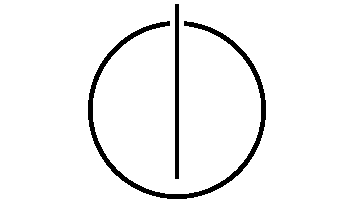
\includegraphics[width=4cm]{styles/informat.png}
  \end{figure}
  
  \end{center}
	\clearemptydoublepage
	% The titlepage for the CAMP report document.
% Included by MAIN.TEX


%--------------------------------------------------
% The title page
%--------------------------------------------------

% correct BCOR - undo at the end !!!
\def\bcorcor{0.15cm}
\addtolength{\hoffset}{\bcorcor}

\thispagestyle{empty}

 \vspace{10mm}
\begin{center}
	       \oTUM{4cm}
	   
	   \vspace{5mm}     
	   \huge FAKULT{\"A}T F{\"U}R INFORMATIK\\ 
	   \vspace{0.5cm}
	 \large DER TECHNISCHEN UNIVERSIT{\"A}T M{\"U}NCHEN\\
        
	\end{center}
		

\vspace{10mm}
\begin{center}

   {\Large \doctype}

  \vspace{10mm}
  
  {\LARGE \title}\\
  
  
  \vspace{10mm}
  
  
  {\LARGE  \titleGer}\\
  
  
  \vspace{10mm}

    %\hfill
    \begin{tabular}{ll}
	   \Large Author:     & \Large \author \\[2mm]
	   \Large Supervisor:    & \Large \supervisor \\[2mm]				
	   \Large Advisor:	& \Large \advisor \\[2mm]
	   \Large Date:       & \Large \date
	 \end{tabular}
	 
	 \vspace{5mm}
	 
	 \begin{figure}[h!]
  \centering
   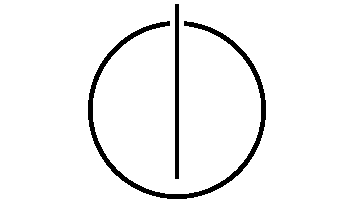
\includegraphics[width=4cm]{styles/informat.png}
  \end{figure}
   

\end{center}

% undo BCOR correction
\addtolength{\hoffset}{\bcorcor}
	\clearemptydoublepage


\thispagestyle{empty}
	\vspace*{0.8\textheight}
	\noindent
	
	I assure the single handed composition of this master's thesis only supported by declared resources.
	
	\vspace{15mm}
	\noindent
	Munich, Germany, \Numberdate \hspace{5cm} \author
\newpage
	\clearemptydoublepage
\phantomsection
\addcontentsline{toc}{chapter}{Acknowledgements}	


%\chapter*{Acknowledgements}

\vspace*{2cm}

\begin{center}
{\Large \bf Acknowledgments}
\end{center}

\vspace{1cm}


I want to express my gratitude to my supervisor, Professor Bernd Br\"ugge for making this project possible. I am especially grateful to my advisor, Juan Haladjian, for finding time and patience to discuss all the ideas that I came up with in the process of writing this thesis.
\vspace{1cm}

I also thank to my beloved friend Deniz Yeltekin for her support during my master study in Munich. She always encouraged me even when I lost my motivation and inspired me with her successes.
\vspace{1cm}

And above all, I would like to dedicate this thesis work to my parents Berrin and Hamdi Yigin. I want to thank my mother for her continual support and words of encouragement, and I want to thank my father for being my inspiration to pursue this field of work and education. I thank to dear my sister Merve Yigin for supporting me. They always believed in me even when I failed. They made a big effort for raising me as a fair and conscientious person.
	% Abstract for the TUM report document
% Included by MAIN.TEX


\clearemptydoublepage
\phantomsection
\addcontentsline{toc}{chapter}{Abstract}	

\vspace*{2cm}
\begin{center}
{\Large \bf Abstract}
\end{center}
\vspace{1cm}


\def\sife {Smart Environment Integration Framework}
\def\TI{TextIt}

\def\seif {Smart Environment Integration Framework}

Electronic textiles (E-Textiles) are a good container for wearable technology and wearable computing specifically to produce activity recognition systems. They enable to use digital components and electronics to embed them into textiles. An activity recognition system built with e-textile can be used in a variety of ares like health monitoring, military and fashion. \\

Since electronic textile is a new concept, it suffers from technology related problems that have not been solved sufficiently; problems such as time consuming data collection, low-level development, unable to test different approaches in an efficient way and no good platform to experience. As a consequence, gathering, observing and testing information from e-textiles and wearable devices poses a challenge, and the development a product is slow and tedious. \\

In this thesis, a complete integrated development environment (IDE) to develop an e-textile product with gathering the data, observing and processing it and testing different algorithms has been proposed. The idea is to combine the playground feature for inexperienced developers and the IDE for e-textiles and wearable devices. User will not need any additional application to get the data from e-textile or wearable devices or any other applications (like WEKA or Matlab) to test and process the signal. \\

The focus of this thesis is on the design and the development of a framework for e-textile development. The framework is a combination of a playground and a conventional IDE. Text based development framework called TextIt that is used for gathering, observing, testing for the e-textile application. The system is developed with playground support to make it easy to enter this area as an inexperienced developer. As the system is able to show the data, have pre-defined algorithms for signal processing and visualize the different test algorithms and compare the results. 

%One page!
%What is the content of your thesis? What are the results, what have you achieved?

%Common mistake:
%This is NOT an appetizer to read your whole thesis. The most interesting things should already be in %the abstract.
	\tableofcontents
  	\clearemptydoublepage

\phantomsection
\addcontentsline{toc}{chapter}{Outline of the Thesis}


\begin{center}
	\huge{Outline of the Thesis} 
\end{center}
\vspace{4mm}
%--------------------------------------------------------------------




\noindent {\scshape Chapter 1: Introduction}  \vspace{1mm}



\noindent The introduction chapter starts with the definition of an e-textile, and a motivation on how it can improve human lives. This chapter describes the challenges that are faced when creating an e-textile product, and proposes a solution for overcoming these challenges.\\

\noindent {\scshape Chapter 2: Requirements Elicitation}  \vspace{1mm}

\noindent  This chapter describes the requirements elicitation which includes the definition of scenarios that drive the development of the TextIT. Based on these scenarios, non-functional requirements are proposed and a functional model with use cases and functional requirements is elaborated. \\

\noindent {\scshape Chapter 3: Analysis}  \vspace{1mm}

\noindent  This chapter provides a description of an analysis model based on the requirements. The model is created to formalize the objects and information that exist in the domain of the e-textile environment. It identifies the entity, boundary and control objects of the TextIt. The created object and sequence diagrams provide a better understanding of the system requirements. As a part of the analysis object model, abstract factory were used for modeling a e-textile environment. By using aa abstract factory pattern tackles a problem of modeling an e-textile communication with multiple messaging types that may execute different set of commands, while each device can use a different communication protocol. \\

\noindent {\scshape Chapter 4: System Design}  \vspace{1mm}

\noindent  This chapter gives a description of the system design model which contains the strategies and practices for designing the TextIt. As a part of the design model, the TextIt is decomposed into smaller subsystems, and the hardware/software mapping is shown. The broker pattern is used for decoupling clients from communication tasks. The broker component is decomposed into sub-components, and the role of each sub-component is shortly described. Finally, persistent data management, software control and boundary conditions are discussed. \\

\noindent {\scshape Chapter 5: Object Design}  \vspace{1mm}

\noindent In this chapter, a description of the components of the broker for controlling the e-textile is given. The interfaces of the components are described in detail. \\

\noindent {\scshape Chapter 6: Conclusion}  \vspace{1mm}

\noindent  This chapter gives a summary of what was done during the course of the thesis. Afterwards, the results are reviewed critically and visions for future work are pointed out. \\


	
% ---------------------------------------------------------------------------
%
% 	Thesis Main Part
%
% ---------------------------------------------------------------------------

\mainmatter
\chapter{Introduction}
\label{chapter:Introduction}



	E-textiles, also known as smart garments, smart clothing, electronic textiles, smart textiles, or smart fabrics, are fabrics that contain embedded digital components (including small computers) and electronics [1]. Simply put, e-textiles are fabrics with electrical characteristics. These electronic devices can be worn on clothes, stored in pockets, held in the hand, or even strapped to the head. E-textiles provide an effective system to store or connect computing elements [12]. 
\\ 
Sensors and low-power processors are now small enough and inexpensive enough to allow the deployment of wireless ad hoc networks for various applications [11]. Recent technological developments have enabled miniaturization; smaller, lower-priced, and lighter chips; wireless sensor networks (WSN); and fiber level research. Thus, e-textiles have emerged, and the research focus has shifted from wearable devices to e-textiles. As in classical electronics, the construction of electronic capabilities in textile fibers requires the use of conducting and semiconducting materials such as conductive textiles [1]. One of the most important issues of e-textiles is that the fibers should be made in a way that they can be insulated and completely washable, so they can be successfully used in clothing manufacture. Fortunately, as a result of fiber level research, a new class of electronic materials has emerged that is more suitable for e-textiles. It is a class of organic electronics materials that can be conducting and semiconducting, and they can be designed as inks and plastics. As a result of this development, woven circuits are now possible to be produced [4]. These woven circuits enable the integration of electronic components in woven e-textiles at the yarn level. Furthermore, in connection to the continuing development of wireless sensor networks, the authors in [9] state that the excitement about this technology is motivated by the several benefits associated with the long-term monitoring, low cost, rapid deployment, self-organization, and flexibility features of WSN. These different technological developments make it possible to create e-textile products with electronic devices that can be worn, bent, washed, and carried without attaching any additional devices. For example, rather than attaching electronic devices to the body with strips, the strips are now the electronic components. Thus, because of all these technological advancements, electronic components can now be integrated into clothing. 
\\
The field of e-textiles can be divided into two main categories:
\begin{itemize}

\item E-textiles with classical electronic devices such as conductors, integrated circuits, LEDs and conventional batteries embedded into garments.
\item E-textiles with electronics integrated directly into the textile substrates.

\end{itemize}

Since textiles play an essential role in human existence, e-textiles possess the potential to be used in many aspects of our lives. Wearable textile products can be utilized in many different areas, including sports, fashion, medicine, rehabilitation, context awareness systems, and social media integration [12]. Representative applications are sports training data acquisition, health monitoring of vital signs, monitoring personnel handling of hazardous materials, tracking the position and the status of soldiers in the field, and monitoring pilot or truck driver fatigue. Furthermore, in the area of rehabilitation as stated in [9], rehabilitation requires continuous supervision during long-term rehabilitation therapy. This continuous supervision increases the workload for physical therapists and medical staff, and it is very expensive for the patients. As a result of such challenges, new sensor-based e-textile solutions have arisen from the need to develop effective, low-cost and easy to use rehabilitation supervision systems. Using e-textile solutions dramatically reduces the cost and size of systems and opens new opportunities [9]. 
\\
Since the field of e-textiles has subcategories, the word e-textile is used to identify a variety of concepts. These concepts include fiber level development, textile sensors, and application development for smart garments (health/rehabilitation, fitness, fashion, maintenance). This thesis focuses on the application level development for e-textiles. In this paper, I present the design and implementation of a framework for rapid development of e-textile applications. 
\\

\section{Problem Statement}

	Smart garments are highly popular among not only researchers but also end users. Despite this interest by both the developers and the end users, only a few developments have exceeded a prototypical level [2]. Moreover, problems still exist that prevent an efficient level of mass production. 
	\\	
	
The basic materials used to produce e-textiles, which are conductive threads and fabrics, have been around for over 1,000 years. However, the e-textile market is still in its infancy, and the quantity of e-textiles being produced is limited. One main reason for and resulting criticism of this limited development and production of e-textiles is the slow and complicated process currently involved. 
\\
	
	
	One of the reasons for the this slow and complicated process is that there are few good high level sources of information or research data to give a practical insight into making e-textile development easier and quicker. The development must go through the following steps: signal receiving, synchronizing, signal filtering, and feature extraction. These essential steps generally need to be done in order to develop an e-textile application. However, when new developers are interested in working in this area, it is hard for them to find solid resources to aid in the development of their applications. Thus, because new developers may not have a comprehensive grasp of the essential steps in e-textile development, they often do not know where to start. 
	\\
	
	 Another reason is that the knowledge that is required to develop e-textiles is complex. The development of e-textiles includes sensor interfaces, synchronization of the sensor signals, and signal filtering [8]. For beginners in the field, it is first required to experiment with the signals, to then review some examples, and finally to use an interactive development tool in order to get some idea about the concept. The IDEs and libraries that are used for e-textile development will be explained in detail in the Related Work section. They focus on either the students that are not professional developers or the experienced developers that have previous experience with e-textiles. These IDEs and libraries do not actually support complex application development since they lack testing, simulation, visualization, and predefined algorithms for machine learning or filtering. All of these procedures should be implemented manually. So that this creates an expectation that users have a deep knowledge about e-textile development, and so they do not really support newcomers to the field.  \\	
	
There is a jungle of libraries and protocols and these libraries and protocols are either vendor specific or operate on the hardware level; for example, the developers must be able to handle the hardware I/0. In this situation, the developers need to start from the beginning by checking hardware level development. This low-level development is another reason for why overall e-textile development is such a slow process. Since there is no good abstractions for the development, users need to work on the hardware elements and develop them manually. This situation creates a time issue for the developers and they felt rushed the development and the problems. Since this low-level of development requires specific information about the device, most developers lack this kind of information, and it is hard to obtain this knowledge quickly and efficiently. Hence, that is the reason development is separated from device in other areas like communication, such as with servers and mobile devices. This device application separation is not available in e-textile science at this point in time.  	\\
	
	Furthermore most developers are not experts in signal processing or activity recognition but want to realize their application concepts using a high level API [2]. Niels Henze et al argue that there is a lack of tool support for application developers and no enough defined APIs within the software and hardware stack that allows developing useful smart garment applications [2]. The hardware that is used to produce e-textile products, like raspberry-pi, Arduino or Intel, does no support for higher level development, there is not enough protocols and libraries to interact with hardware components. The problem is there is no application layer in the e-textile development yet. (Fig. 1.1). As a result, all the communications with hardware ,such as reading the data from sensors or writing to actuators, are needed to be done by the developers. This situation makes building more complex systems even more harder. Like in development of mobile or desktop application, in the development of e-textile also requires for APIs that support more complex commonly used functions or functionality such as data mining and machine learning. Unfortunately in the current situation there is no tool support for application developers and no defined APIs within the software [2]. The development is on specific devices that the libraries or protocols are designed for. This makes an application is specific to that devices or vendors. All the signal-processing algorithms, signal synchronization or filtering methods are developed specific to the device because all the read inputs and write outputs are specifically designed according to used hardware. Thus the knowledge about developing on hardware is required from the developers. Since expecting a good knowledge on hardware development is not realistic, there are researches on creating a top development level on hardware are going on [2,4,5,8,9]. \\

	Most of the development environments, which are used to test different system variants, are not suitable for actually running applications [8]. These environments are dependent upon custom engines or libraries. For this reason, in order to test different systems, implementing an actual e-textile application for specific device is necessary. In order to do this, developing selected algorithms in an appropriate programming language and then distributing them to specific devices are necessary. Relevant issues in this process include sensor interfaces, synchronization of the signals, and optimizing for specific devices. Although the applications are similar, when the developers want to test them on other devices, since all the implementations are done for a specific device, the same development has to be done from the beginning for any different hardware.  \\
	

	In addition to all of these problems, developing e-textiles is a complicated process. E-textile development is similar to distributed systems. It is hard to communicate and synchronize between different sensors. Moreover, as stated before, it is hard to simulate the application before actual implementation; therefore, it is not easy to test a system. Developers may not know which algorithms to use in their application. For example, just for filtering alone, there are more than twenty-four algorithms that can be used for smoothing the signals [10]. In order to find the best one, it requires several phases of testing. Also, the algorithms change according to the data and the sensor. Since there is no easy way to simulate the data and test them with different algorithms to find the best ones, the developers need to implement every algorithm that they want to compare, in order to find the suitable one. The developers need to collect the data again, apply the algorithm, see the results, and compare them. This cycle needs to be done for different algorithms to compare the results and find the appropriate ones. They cannot change the algorithm in the apply algorithm phase. If they want to test a different algorithm, they need to start the process from the beginning. This is a time-consuming process when the system is more complex. 


\insertfigure{images/mcan/Introduction/layered.png}{Presented Development Layer}{UserFixtures}{0.30}



\section{Related Work}

The following sections provide the summary of proposed related framework to work on e-textile development.

\subsection{E-textile Generic Environments}

In this section the generic environments, that are created to create an abstraction for e-textile systems, are explained in detail. \\ 

The CRN Toolbox enables fast implementation of activity and context recognition systems, featuring mechanisms for distributed processing and support for mobile and wearable devices. It is a tool set specifically optimized for implementing multimodal, distributed activity and context recognition systems running on Posix operating systems. The CRN Toolbox contains a collection of ready-to-use algorithms (signal processing, pattern classification, and so on). Another important feature is the ability to interface conventional simulation environments such as WEKA (Waikato Environment for Knowledge Analysis, www.cs.waikato. ac.nz/~ml). The concepts the CRN Toolbox uses are graphical programming, data driven computation, parameterizable libraries, and distribution. \\

TinyOS is an open-source operating system designed for low-power wireless devices, such a sensor networks, ubiquitous computing, personal area networks, smart buildings and smart meters. TinyOS provides useful software abstractions of the underlying device hardware. TinyOS is especially useful for microcontroller-based devices that have sensors and/or networking capabilities. It is developed to make a layer on top of the hardware so that the Os separately runs the applications from hardware.


\subsection{E-textile Frameworks and Platforms}
In this section the platforms and frameworks with collection of different algorithms to work on e-textile data.\\

Matlab is a High-level language for numerical computation, visualization, and application development. It has predefined mathematical functions for linear algebra, statistics, Fourier analysis, filtering, optimization, numerical integration, and solving ordinary differential equations. It supports Built-in graphics for visualizing data and tools for creating custom plots. \\

Weka is a collection of machine learning algorithms for data mining tasks. The algorithms can either be applied directly to a data-set or called from your own Java code. Weka contains tools for data pre-processing, classification, regression, clustering, association rules, and visualization. It is also well-suited for developing new machine learning schemes. Advantages of Weka include, free availability under the GNU General Public License, portability, since it is fully implemented in the Java programming language and thus runs on almost any modern computing platform, a comprehensive collection of data pre-processing and modeling techniques, ease of use due to its graphical user interfaces. \\

\subsection{E-textile Development Environments}

The following section provides the summary of related development environments to create e-textiles. \\ 

	There are different models in the market right now to produce wearable or e-textile devices. As an example there are; Arduino Lilypad, which is cheap board and has low energy consumption. It is designed to build soft interactive textiles. Raspberry-pi is cheap, bigger than Arduino Lilypad, powerful and has high-energy consumption. Intel Edison has very powerful microprocessor, Wi-Fi and Bluetooth low-level energy but bulky design. Beaglebone is very similar to Raspberry-pi, has a size of a credit card. \\


There are different development environments specifically for almost every other hardware that is listed above.  Arduino IDE is a text based programming language for Arduino hardware. Its language is similar to C++. It has 1-click deployment feature but no debugging.  \\

In Gadgeteer hardware structure is defined visually (components and their connections). Automatic code is generated based on visually defined structure. It has debugging feature and also text based programming in C\#.  \\

Espruino IDE is Google Chrome plug-in. It is a script and block based programming language. It can upload automatically to the Espruino microprocessor. \\

Cloud9 is another browser based collaborative development environment. Version management integrated in the environment. It is also text based programming language in Node\.js and Javascript. Node-Red is visual flow based programming environment based on Node\.js. It runs as a Web Server. Programs can be created from any browser and offers components with higher-level features such as Tweeting, Mail. It can be used to connect the beans to the cloud and define behaviors such as alerting over email when temperature drops below some level. \\

I\*CATch is a hybrid with visual and textual programming environment for Arduino based micro-controllers. Its targets are children and novices. It is based on bus architecture. And it is available to plug and play programming blocks and connect them to denoted program flow.  \\

Fritzing is open source software for documenting and prototyping hardware involving micro-controllers sensors and actuators. Their purpose is to help hobbyists, designer and artists to produce their designs. It supports many components including micro-controllers, sensors, actuators and smaller parts such as resistors and connectivity modules. It has functionality to export the design in order to share it with other users. SAM is visual flow based programming environment for the SAM Kit. It can translate visual representation into code that can be uploaded wirelessly to the boards. \\

RUNES (Reconfigurable Ubiquitous Networked Embedded Systems), is a project to enable the creation of large scale, widely distributed, heterogeneous networked embedded e-textile systems that interoperate and adapt to their environments. RUNES aims to provide an adaptive middleware platform and application development tools that allow programmers the flexibility to interact with the environment where necessary. It also offers a level of abstraction that facilitates ease of application construction and use. This will allow for a dramatic cut in the cost of new application development and a much faster time to market. \\

\subsection{Interactive Development Environments for Teaching}

Swift playground is introduced by Apple to make swift learning more interactive, effective and fun. Playground makes writing Swift code incredibly simple and fun [13]. Whenever the users enter a line of code, the result appears immediately. For immediate result the Swift playground uses REPL (read-eval-print-loop) approach. Thus the playground does not require any compiling and keep listening the input from the users. The playground can be used for designing a new algorithm by watching its results every step, create new tests by verifying the work before applying into the test suite and experimenting with new APIs. \\

Khan Academy has also launched an online development environment for teaching purpose. This online environment contains a set of tutorials based on the JavaScript and Processing languages and supports live coding environment like Swift playground, where the program updates the output as the programmers write. \\

Processing is an open source programming language built for teaching the fundamentals of computer programming in a visual context and to serve as the foundation for electronic sketchbooks. One of the stated aims of Processing is to act as a tool to get non-programmers started with programming, through the instant gratification of visual feedback. \\

Greenfoot is an interactive Java development environment for also educational purposes. Its main focuses are two-dimensional graphical applications like simulations and games. The aim of Greenfoot is to give programming education (object-oriented programming) at high school and early university level. \\

Bluej is another Java environment specifically for first year college students. It is developed to eliminate some of Java's complex syntax and represents the object/class relationship visually. Special emphasis is placed in Bluej on visualization and interaction techniques to create an interactive environment to encourage experimentation and exploration. \\

Bret Victor, the owner of the work that was cited as an inspiration for the Khan system, emphasizes that; the goals of a programming system should be: 

\begin{itemize}

\item to support and encourage powerful ways of thinking
\item to enable programmers to see and understand the execution of their programs

\end{itemize}

As a live coding example Processing do not address any of these goals [14]. Bret Victor further criticizes JavaScript and Processing as a poorly-designed languages since they do not support ways of thinking and ignores learning process. Without these goals a live coding environments are worthless.

\section{Solution}

According to problems that are described in section 1.1, an interactive e-textile development environment, so called TextIt, is proposed as a solution in order to increase the speed of development and as a result more developers may join to production even they do not have previous knowledge. \\ 


The solution of development environment that is proposed is to create some kind of an e-textile playground for the developers. In that development environment, developers may get some sample data or receive the real data from e-textile products and have predefined components, which are required to process data, so that they can try their own application ideas by using the components. These components have to be extracted according to current market needs. In the e-textile applications there are some common components that are used several times like Bluetooth communication, signal processing, filtering, machine learning and etc. Since these steps are common and there are some standardized solutions for that problem, the environment should support pre-defined solutions for those common problems. Implementing those components for every application is a wasted effort and money especially they do not change over time. Moreover since the developers are required to test and experiment with different algorithms before the actual implementation, the development environment can solve this problem by providing the algorithms that the developers need and can show the result of the algorithms. By this approach the developers can see the effect of the algorithms and choose the best one for their applications and use it for actual implementation. This support for pre-defined components helps developers to explore more and be more free. With this approach rather worrying about how to implement the algorithms, the developers can focus on the big picture and be more imaginative and think about more complex applications. Focusing on the actual application and thinking about what can be done rather than how can be done can help e-textile to be more innovative and can address the problems of the market. \\

As a result, to realize the solution of a development environment for e-textiles, needed APIs, pre-defined algorithms and components are required to be identified. The purpose to collect those requirements under one environment is to support developers to easily access the resources specifically for e-textile development. The aims of this e-textile environment, so called TextIt \ in this thesis, are to speed up the development of e-textiles, make it available for many developers that have different knowledge background and make the applications hardware independent to extend its usage area.

\def\kneehapp {KneeHapp}


\chapter{Requirements Elicitation}
	
	The requirements elicitation chapter provides a description of the overall use of the system and defines the requirements that the system has to meet. The requirements are extracted from the project \kneehapp. In order to identify the requirements the project KneeHapp is developed with the current technologies that are available to develop smart garments. After using the available e-textile development environments and frameworks, the missing pieces are identified.  \kneehapp  project is developed in TUM iOS praktikum with Prof. Bern Br\"uge and sport traumatology expert Dr. J\"urgen H\"oher in 2014. Moreover the participants of this project were computer science students and had not previous knowledge about e-textile development. This made us also see the barriers and challenges for beginners to e-textile development. With \kneehapp project we had the chance to work on a real e-textile project and see the current status and the drawbacks of the area. The most of the requirements are extracted by our observations. The requirements are extracted from the scenarios described below. Extracted requirements are divided into two categories: \textbf{functional requirements} and \textbf{non-functional requirements}. Functional requirements describe the interaction between the system and its environment, independent of its implementation \cite{Bruegge2004}. Non-functional requirements refer to user requirements that are not directly related to the functional behavior of the system \cite{Bruegge2004}.

	
\section{Project \kneehapp}

The rupture of the anterior cruciate ligament (ACL) of the knee is a severe injury. ACL ruptures are mainly the result of sports related injuries such as football, basketball, handball, and contact sports. An intense rehabilitation period is necessary to bring the individual back to physical activities and the desired sports. The rehabilitation of the knee often includes physical therapy and strength exercises. The progress and the success of the rehabilitation measures are currently not well documented. The goal of this project is to develop a system that would allow patients to record their rehabilitation progress without the need of a doctor or physiotherapist. During the Summer Semester 2014 we, six TUM students, developed a smart bandage (Kangaroo Bandage) and iPad application (\kneehapp) that measure performance parameters while the patient performs the rehabilitation exercises. The smart bandage was consisted of two Arduino devices and the devices were put in to the knee bandage. One of the exercises that were supported was "One Leg Hop". The one Leg Hop is an exercise in which the patient jumps forward as far as he/she can with only one leg. Then the algorithm calculates the duration of the hop. The other exercise was "Side Hops". In this exercise patient should jump right and left as many times as he/she can in the given time. Then the algorithm calculates the number of the hops from accelerometer data.


\section{Use Cases}

The requirements are extracted by use cases and they also serve to describe the functionality of the system from the users point of view \cite{Bruegge2004}.

\subsection{	One Leg Hop}

One Leg Hop is the exercise that the patient should jump as far as he/she can, then the smart garment should calculate the duration of the hop by processing the acceloremeter data. 
Figure 2.1 shows the linear accelerometer data from the y and z-axis corresponding to a one-leg hop. Even for human eyes it is not easy to read this accelerometer signal. There are one maximum peak and two minimum peaks in the signal. Thus without further observations, one can not conclude which points corresponds to jumping and landing. So that we could take the time difference between these two points. It was not really possible to implement the algorithm before really understanding the signal and knowing which points to take. We made several iterations of jumping, collecting the data, video recording of the jump, using different filtering methods, using different feature extraction methods. Unfortunately at the end we found measuring the duration of a hop from accelerometer signal challenging due to the fact that hops occur very quickly (an average hop lasts around 0.22 seconds) and there are so many noise because of the leg shaking. One possible solution we proposed was using an insole with integrated pressure sensors. We thought that it could be more easier to detect when the user leaves the ground and lands the ground by using insole with pressure sensor. Figure 2.2 shows the insole and its hardware. Figure 2.3 shows the signal produced by the pressure sensors during a one-leg hop. We could then determine whether the user is on the ground or in the air using a threshold. 

\insertfigure{images/mcan/Requirement/oneleghop-acc.png}{One Leg Hop with Accelerometer Data}{UserFixtures}{0.40}
\insertfigure{images/mcan/Requirement/insole.png}{Insole - Pressure Sensor}{UserFixtures}{0.40}
\insertfigure{images/mcan/Requirement/oneleghop-insole.png}{One Leg Hop with Pressure Sensor}{UserFixtures}{0.40}

\subsection{	Side Hops}

Side Hops is the exercise that the patient should jump right and left as many times as he/she can in the given time. Then our smart garment should calculate the number of jumps. This was rather an easier exercise than the One Leg Hop to calculate. To given an idea about how the signal looks like, the example linear acceleration on the horizontal axis for 7 side hops is given in Figure 2.4. This was rather cleaner and easier to understand when compared to One Leg Hop exercise signal. The number of jumps are clear for human eyes, as the peaks indicates the jumps. However for the algorithm to calculate the number of the jumps, we needed to filter the signal from the noise. In order to eliminate noise in the signal, we applied several iterations of a low-pass filter until the signal's standard deviation became smaller than a specific threshold. We called this threshold low-pass filter threshold. We found the optimal low-pass filter threshold to vary depending on the algorithms used for calculating the jump duration. We tested the RC low-pass filter with a time constant T = 0.25 and a weighted moving average filter with coefficients [1/4 1/2 1/4]. After filtering the signal, we used a peak detection algorithm to count the high and low peaks in the signal. A naive peak detection algorithm counted also local maxima as hops in the signal, resulting in more side hops being counted. To overcome this issue we analyzed the surroundings of a peak. If the peak is larger enough than its surroundings, the peak is counted as a hop. We called this factor peak threshold. We found the peak threshold leading to most accurate results to depend on the filtering algorithm used. Figure 2.5 shows the same 7 hops after applying three iterations of the RC filter and running the peak detection algorithm.


\insertfigure{images/mcan/Requirement/sidehop-raw.png}{Side Hop Raw Data}{UserFixtures}{0.40}
\insertfigure{images/mcan/Requirement/sidehop-filtered.png}{Side Hop Filtered Data}{UserFixtures}{0.40}


\section{Requirements}
			
In this section requirements are presented. Requirements are collected into 3 main parts; gathering, observing and testing the data. Paul Lukowicz et al. argues the requirements for e-textile environments can be listed as, a collection of ready-to-use algorithms (signal processing, pattern classification, and so on), synchronization, merging, and splitting of data streams. The environment should include I/O device readers and writers, filtering and classification algorithms, and components for splitting, merging, and synchronizing data streams. Also a visualizer is a must to show the data to user. Thus it would be easier to work on the data. 

\subsubsection{Observation 1: Gathering}


In our case since we did not know how the signal looks like, first of all we needed to collect sufficient amount of sample data to really understand the signal and discover what peaks, curves, numbers and points actually mean in the context. Collecting sufficient amount of data is the important key before the actual implementation because first we need to understand the data and the problem before proposing the solution to that. Understanding the signal by gathering data is required since the developers did not have previous knowledge about e-textile field and know how the actual data looks like. In our project for this purpose, we developed a mini application to record all the acceleration and gyroscope data. After all the collection process was done, we needed to transfer to data into an environment in which we process the signal. Although it might sound as an easy process it took several full days to only collect 10 jumps from users. 
	
	
\subsubsection{Observation 2: Observing}


After the collection of the data, the signal was passed to another environment in which it was processed. As mentioned before, since the developers had not had any previous knowledge about the data, it was necessary to show how actually the signal looks to give an overview about the problem. Then we could understand the signal better and decide what was needed to process the signal (filtering, feature extraction, data mining, machine learning). In our case we used different environments and frameworks ,like WEKA, Matlab, Octave as desktop applications and JBChartView, iOS Chart etc. for iOS integration, to visualize the exercise signal. To try every different framework we had implemented them in our project to see which ones gave the better solution for our application. Because every framework is suitable for different purposes, it took quite a time to find the best one for our needs. It was necessary to show not only the original signal to developer but also how it looked like after every manipulation the developer made to process the data and make it more understandable. With this approach we could see what effects every algorithm had. Also we had the same approach when deciding the filtering and feature extraction methods to use. In our project we implemented different filtering and feature extraction methods and applied them to data sequentially and noted the results of the methods.


\subsubsection{Observation 3: Testing}


As every algorithm has different effects on the signal, we wanted to see which one had the best results for our project. In our case we manually took the result of different methods and compared them with our references. Then we created a table to see which ones we should use. To find the appropriate methods, it required several iterations of gathering, observing and testing. Since only one iteration takes significant amount of time, repeating this loop was a time consuming process. It would be easier if we could have defined the different test cases to run and the references to compare with to the development environment, then the result returned as an excel like table to present the final results of different test cases and the comparison of the accuracies.

\subsection{Functional Requirements}
The following subsection defines functional requirements identified from the previously shown use cases.

\subsubsection{FR1: Data Gathering}
\textit\ should allow the user to receive data from an external e-textile device.

\subsubsection{FR2: Data Observing}
\textit\ should allow the user to visualize the data.

\subsubsection{FR3: Data Testing}
\textit\ should show the result of different test cases and the comparison of their accuracies. 

\subsubsection{FR4: Test Case Management}
\textit\ should allow the user to create and to run different test cases.

\subsubsection{FR5: Pre-defined Algorithms}
\textit\ should allow the user to use pre-defined algorithms.

\subsubsection{FR6: Live Coding}
\textit\ should interpret the user input live with REPL (read eval print loop) approach.



\subsection{Non-functional Requirements}

In the following subsection, the non-functional requirements of \textit\ will be described.

\subsubsection{NF1: E-textile Device Independence} 
\textit\ should provide suport to receive from different e-textile products.

\subsubsection{NF2: Extendibility with Respect to Algorithms} 
\textit\ should support the addition of defined algorithms.

\subsubsection{NF6: Response Time}
\textit\ should provide system feedback within 5 seconds (an error message in case of an error or a message about a successful execution of a command)

\subsubsection{NF7: Robustness}
Invalid user input shall not cause any disruption in the functioning of \textit.

\subsubsection{NF11: Operating System}

\textit\ should run on MAC OS. 


\section{Related Work}

The following sections provide the summary of proposed related framework to work on e-textile development.

\subsection{E-textile Generic Environments}

In this section the generic environments, that are created to create an abstraction for e-textile systems, are explained in detail. \\ 

The CRN Toolbox enables fast implementation of activity and context recognition systems, featuring mechanisms for distributed processing and support for mobile and wearable devices. It is a tool set specifically optimized for implementing multimodal, distributed activity and context recognition systems running on Posix operating systems. The CRN Toolbox contains a collection of ready-to-use algorithms (signal processing, pattern classification, and so on). Another important feature is the ability to interface conventional simulation environments such as WEKA (Waikato Environment for Knowledge Analysis, www.cs.waikato. ac.nz/~ml). The concepts the CRN Toolbox uses are graphical programming, data driven computation, parameterizable libraries, and distribution. \\

TinyOS is an open-source operating system designed for low-power wireless devices, such a sensor networks, ubiquitous computing, personal area networks, smart buildings and smart meters. TinyOS provides useful software abstractions of the underlying device hardware. TinyOS is especially useful for microcontroller-based devices that have sensors and/or networking capabilities. It is developed to make a layer on top of the hardware so that the Os separately runs the applications from hardware.


\subsection{E-textile Frameworks and Platforms}
In this section the platforms and frameworks with collection of different algorithms to work on e-textile data.\\

Matlab is a High-level language for numerical computation, visualization, and application development. It has predefined mathematical functions for linear algebra, statistics, Fourier analysis, filtering, optimization, numerical integration, and solving ordinary differential equations. It supports Built-in graphics for visualizing data and tools for creating custom plots. \\

Weka is a collection of machine learning algorithms for data mining tasks. The algorithms can either be applied directly to a data-set or called from your own Java code. Weka contains tools for data pre-processing, classification, regression, clustering, association rules, and visualization. It is also well-suited for developing new machine learning schemes. Advantages of Weka include, free availability under the GNU General Public License, portability, since it is fully implemented in the Java programming language and thus runs on almost any modern computing platform, a comprehensive collection of data pre-processing and modeling techniques, ease of use due to its graphical user interfaces. \\

\subsection{E-textile Development Environments}

The following section provides the summary of related development environments to create e-textiles. \\ 

	There are different models in the market right now to produce wearable or e-textile devices. As an example there are; Arduino Lilypad, which is cheap board and has low energy consumption. It is designed to build soft interactive textiles. Raspberry-pi is cheap, bigger than Arduino Lilypad, powerful and has high-energy consumption. Intel Edison has very powerful microprocessor, Wi-Fi and Bluetooth low-level energy but bulky design. Beaglebone is very similar to Raspberry-pi, has a size of a credit card. \\


There are different development environments specifically for almost every other hardware that is listed above.  Arduino IDE is a text based programming language for Arduino hardware. Its language is similar to C++. It has 1-click deployment feature but no debugging.  \\

In Gadgeteer hardware structure is defined visually (components and their connections). Automatic code is generated based on visually defined structure. It has debugging feature and also text based programming in C\#.  \\

Espruino IDE is Google Chrome plug-in. It is a script and block based programming language. It can upload automatically to the Espruino microprocessor. \\

Cloud9 is another browser based collaborative development environment. Version management integrated in the environment. It is also text based programming language in Node\.js and Javascript. Node-Red is visual flow based programming environment based on Node\.js. It runs as a Web Server. Programs can be created from any browser and offers components with higher-level features such as Tweeting, Mail. It can be used to connect the beans to the cloud and define behaviors such as alerting over email when temperature drops below some level. \\

I\*CATch is a hybrid with visual and textual programming environment for Arduino based micro-controllers. Its targets are children and novices. It is based on bus architecture. And it is available to plug and play programming blocks and connect them to denoted program flow.  \\

Fritzing is open source software for documenting and prototyping hardware involving micro-controllers sensors and actuators. Their purpose is to help hobbyists, designer and artists to produce their designs. It supports many components including micro-controllers, sensors, actuators and smaller parts such as resistors and connectivity modules. It has functionality to export the design in order to share it with other users. SAM is visual flow based programming environment for the SAM Kit. It can translate visual representation into code that can be uploaded wirelessly to the boards. \\

RUNES (Reconfigurable Ubiquitous Networked Embedded Systems), is a project to enable the creation of large scale, widely distributed, heterogeneous networked embedded e-textile systems that interoperate and adapt to their environments. RUNES aims to provide an adaptive middleware platform and application development tools that allow programmers the flexibility to interact with the environment where necessary. It also offers a level of abstraction that facilitates ease of application construction and use. This will allow for a dramatic cut in the cost of new application development and a much faster time to market. \\

\subsection{Interactive Development Environments for Teaching}

Swift playground is introduced by Apple to make swift learning more interactive, effective and fun. Playground makes writing Swift code incredibly simple and fun [13]. Whenever the users enter a line of code, the result appears immediately. For immediate result the Swift playground uses REPL (read-eval-print-loop) approach. Thus the playground does not require any compiling and keep listening the input from the users. The playground can be used for designing a new algorithm by watching its results every step, create new tests by verifying the work before applying into the test suite and experimenting with new APIs. \\

Khan Academy has also launched an online development environment for teaching purpose. This online environment contains a set of tutorials based on the JavaScript and Processing languages and supports live coding environment like Swift playground, where the program updates the output as the programmers write. \\

Processing is an open source programming language built for teaching the fundamentals of computer programming in a visual context and to serve as the foundation for electronic sketchbooks. One of the stated aims of Processing is to act as a tool to get non-programmers started with programming, through the instant gratification of visual feedback. \\

Greenfoot is an interactive Java development environment for also educational purposes. Its main focuses are two-dimensional graphical applications like simulations and games. The aim of Greenfoot is to give programming education (object-oriented programming) at high school and early university level. \\

Bluej is another Java environment specifically for first year college students. It is developed to eliminate some of Java's complex syntax and represents the object/class relationship visually. Special emphasis is placed in Bluej on visualization and interaction techniques to create an interactive environment to encourage experimentation and exploration. \\

Bret Victor, the owner of the work that was cited as an inspiration for the Khan system, emphasizes that; the goals of a programming system should be: 

\begin{itemize}

\item to support and encourage powerful ways of thinking
\item to enable programmers to see and understand the execution of their programs

\end{itemize}

As a live coding example Processing do not address any of these goals [14]. Bret Victor further criticizes JavaScript and Processing as a poorly-designed languages since they do not support ways of thinking and ignores learning process. Without these goals a live coding environments are worthless.

\chapter{Analysis}

	In this chapter, an analysis model based on the requirements elicitation will be presented. The main purpose of the analysis model is to structure and formalize the elicited requirements and to identify the objects that exist in the application domain. An analysis model is composed of three individual models: a \textbf{functional model}, represented by the use cases and scenarios, an \textbf{analysis object model}, represented by the class and object diagrams and a \textbf{dynamic model}, represented by the state machine and sequence diagrams \cite{Bruegge2004}. The functional model was presented in the previous chapter. To complete the system requirements analysis model, object and sequence diagrams will be presented.

	
\section{Analysis Object Model}

	The application consists of 3 stages; gathering, observing, testing. For simplicity and easy to read these categories will be explained separately. Firstly, the analysis object model of the gathering, which includes communication with the hardware and collecting the data, is shown in the UML class diagrams and is developed iteratively in the following section. The initial model is shown in figure \ref{oldCommunicationDiagram}.

\insertfigure{images/mcan/Analysis/oldCommunicationDiagram.jpg}{Old Analysis Object Model}{oldCommunicationDiagram}{1.00}


%used Firmata protocol
%composite pattern 
%template/strategy pattern

In this model the software can connect to different kinds of e-textile components. Also in an e-textile component there can be different sub-components which have different functionality (actuators, sensors), addresses, registers and pins. The communication can be different between the actual component and the sub-components so the correct command should be sent. Even the communication through these different e-textile components can vary depending on the manufacturers. In addition to this, the two same devices can send the information in a different way, so that it has to be parsed differently. As it is stated in the requirements elicitation the system should be extendable, it should connect to different devices and the communication shouldn't be device dependent. \\

Moreover, the initial model is designed to only get acceloremeter and gyroscope values (I2C values). However one e-textile component can have not only I2C messages but also Analog and Digital sensors. In order to tackle this issue and make the communication device independent, the well-known and widely used Firmata protocol is used in this project.\\

Firmata protocol allows the ability to communicate with the devices without knowing the model of the device and it ensures that the message that is received will be in the same format. The Firmata protocol proposes three different communication ways. For analog sensors it has Analog messages, for digital sensors there are Digital messages and for acceloremeter and gyroscope value it has I2C messages. The way to communicate and the response received from this communication include different meanings and different information. Yet in all communication type there needs to be a name of the data to call it later in the code, the default name is given according to message types. Because the data type changes based on the communication type in abstract class the data is shown as a generic type AnyObject. Later this will be implemented accordingly to the communication type. Although it is an array of numbers in Digital and Analog messages, it is a double array of numbers in I2C. The reason of being a double array in I2C is the e-textile component returns different information from different sub-components at the same time. In every message that is received has an acceleration x,y,z and gyroscope values of x,y,z. \\

The data is saved to a file after collecting data is done. In order to save the messages and their data to a file the abstract class implements Printable class. This interface enables to have a description method to return a string representation of information the class has. Since the types have different data types and different variables the description of the classes should be also different. The template pattern is used to solve that problem by allowing having different implementations of description method \cite{GoF}. So that the description algorithm can be overridden by subclass to have a different behaviors by still following the overall flow. \\

To get the data or the description of every messages one by one can be time consuming and redundant. In those cases those different sub classes of messages can be treated as a single instance of an object since they all support the same variables. The composite pattern is used for this issue. The composite patterns allows users to treat group of different messages as a single object \cite{GoF}. \\
	
	The second iteration is presented in figure \ref{CommunicationDiagram2} \\

\insertfigure{images/mcan/Analysis/CommunicationDiagram.jpg}{Analysis Object Model}{CommunicationDiagram2}{1.00}

The 3 different communication types use different protocols to communicate with the e-textile component. They send different messages and different inputs like pin number, address number or register number. There is a problem of having multiple communication types and they all contain different variables with different protocols. To achieve the problem an abstract factory pattern is used \cite{GoF}. In figure in figure \ref{CommunicationDiagram2}the abstract factory object is Communication Type Factory object. The 3 different communication types are the concrete objects that contain the necessary information to success the communication. \\

Another functionality of the system is observing data. The meaning of observing data is visualizing the data, manipulating it, applying filter methods, feature extraction methods or machine learning methods and visualizing it again. So that the users can extract the necessary information that they need and in every step they can follow the process and see how the data is changed. \\

To support users when they want to manipulate the data or apply some machine learning methods, they are pre-defined in the application so that these components are ready to use. The user can create an actual object from the components and can use it by giving the necessary inputs. Here in this model there are multiple components that are added to application. The components is the abstract object for the feature extraction, filter and machine learning methods. In deed they are also abstract objects and they include the actual implementation of the methods like; peak-detection algorithm, low-pass filter algorithm or k-nearest-neighbor algorithm \ref{ComponentDiagram1}. \\

In this model using an Abstract Factory pattern is considered, but for the simplicity to the user it is not used. Since the users are mostly developers; it is left as an Object-Oriented programming. The user can create the objects by using new() methods and start using them. The application itself is an IDE and the users are actually programming. To give freedom to the users and for the simplicity, abstract factory pattern is not used here. \\

\insertfigure{images/mcan/Analysis/ComponentDiagram.jpg}{Component Diagram}{ComponentDiagram1}{0.80}

At the final stage there is testing  part to see how different algorithms effect the data and gives the best result. Here to get the accuracy the user should have a reference to compare. For example a jump count in Side-hops use case. The each component algorithms have different effects on the data. So here the user can create multiple use cases with different component algorithms and get the result of the each test cases and see the final accuracy in a table format. Easily the user should compare and see the best test case by comparing the accuracy of the use cases on the table \ref{TestDiagram}. 

\insertfigure{images/mcan/Analysis/TestDiagram.jpg}{Testing Diagram}{TestDiagram}{0.80}














\chapter{System Design}
	The system design chapter focuses on transforming the previously described requirements analysis model into a system design model. The system design model contains a description of design goals, subsystem decomposition and strategies (hardware/software mapping, persistent data management, access control policy) for building the system. The goal of this chapter is to describe the system decomposition and to give a clear description of the strategies that are to be used for building the system. 
	
\section{Design Goals}
The system design of TextIt was based on the following design goals:

%ble-firmata, communication model
%communication message selection
%gathering saving displaying data
%JS Runner
%plug-in pattern Interactex
%left pannel, toolbar, menubar, debug view
%Components model
%pre-defined methods?
%user added methods (parser. test cases)

	%ble-firmata, communication model
	\subsubsection{Support of Different E-Textile Hardware} 
Different hardware manufacturers have different communication protocols. Even on the same hardware the messages getting values from different analog, digital or I2C messages can differentiate. To overcome the communication problem and to make it more device independent, the system has been developed with Firmata protocol. This Firmata protocol is implemented in Communication Manager. The component contains different messaging implementations while providing a uniform interface for the interactions. More information about this component is given in \textit{Object Design} chapter.\\

The Firmata protocol helps to overcome lack of uniform communication problem. In addition to this in order to connect to hardware at the first place, the BLE (Bluetooth Low Energy) library has been used. The BLE library helps to connect to hardware and start communication via Bluetooth 4.0. So that the system can connect to any hardware ,that is supporting BLE feature, wirelessly.

	To Separate system communication functionality from the main application functionality, the communication manager is used as a broker that isolates communication-related concerns (Broker Pattern).
	
	%communication message selection
	\subsubsection{Selection of Different Communication Message Types} 
The system should enable adding, removing, modification of different message types to communicate with the connected hardware. The Firmata protocol supports 3 different message types. The users should be able select which message types they want to use and how many different hardware components they want to communicate. For example there might be a case where the user wants to communicate via Analog Message with 3 different components on the hardware. This is accomplished by introducing E-textile Communication Selector Controller. In this controller user can add or remove by dragging and dropping the message types and identifies their pin, register, address number. So that the user can connect to any component on the e-textile hardware. More information about this component is given in \textit{Object Design} chapter.
	
	%gathering saving displaying data
	\subsubsection{Saving ad Displaying the Incoming Data From E-Textile} 
	TextIt should help to users to understand which data, users are receiving. It is stated that the users can get 3 different messages (data) from many different hardware components. In order to identify which message type sends what kind of data, the system displays the message data to users while receiving the data. So that the users can see the data, that is currently receiving. This may help users to see whether it is the data that they want to get and whether there is a problem with the data before continuing working on the data. \\
	
	Moreover to use the data later on and keep it persistently, users can save their data under the given file. The system enables to enter the file name and an option to save the data. This is accomplished by introducing Gathering Window Controller right after the message types are selected. More information about this component is given in \textit{Object Design} chapter.
	
	%JS Runner
	\subsubsection{Supporting Scripting Language} 
	The system should interpret a scripting language to enable its user to code their own program and use the tools. To achieve interpreting the user input live with REPL (read eval print loop) approach, using a light scripting language is decided. REPL (read eval print loop) method is chosen to support playground feature for beginner programmers, so that the system is more interactive and return the result of the code immediately. This encourages the inexperienced users when they see their result or problems immediately. Moreover in a result the system is light, easy to use, returns immediate results, and has a modern look rather than having an old way of compiler approach. For this feature JavaScript Runner component is added to the system. The reason choosing JavaScript and more information will be explained in \textit{Object Design} chapter.
	
	%plug-in pattern Interactex
	\subsubsection{Should Connect and Push User Defined Code to Interactex Program} 
	Interactex is the visual programming version of TextIt, and developed by my supervisor \advisor . They target the similar goals for development of e-textile programming. TextIt can support the Interactex where it has some drawbacks because of the visual programming. In TextIt users can program their own custom algorithms and push their own methods to Interactex. The system supports this communication with Interactex and push the user defined methods. To achieve this feature plug-in pattern is used. 
	
	%left pannel, toolbar, menubar, debug view
	\subsubsection{Supporting Basic Features of Integrated Development Environment} 
	The system is designed to be an Integrated Development Environment(IDE) for e-textile development. Thus there are some common features that IDEs are supporting. As they can be found in many IDEs, the left panel is reserved for folder view. So that users can go through different files or folders in the project folder. The system also supports creating a new file/folder. 
	
	In the toolbar not only to the classic functions are added like text size, font and color buttons but also some new functions that are specific to the system is like record button for connecting to e-textile hardware and getting the data from it and push button for sending the user defined code to other platforms like Interactex.

	Since it is an IDE and allows users to program the debugger view is attached at the bottom of the view traditionally. Whenever there is a result of user code or an exception it is immediately printed to debugger view.	
	
	In order to keep integrity between models and view the widely used Model View Controller architectural design pattern is used. So that Model subsystem is responsible for application domain knowledge, View subsystem is Responsible for displaying data to the user and Controller subsystem is responsible for sequence of interactions with the user and notifying views of changes in the model.

	%Components model
	\subsubsection{Ready to Use E-Textile Development Components and Pre-defined Functions}
	The system contains some ready to use components to hep users to develop their e-textile program in an efficient way. These components are the methods that are widely used in e-textile development like signal smoothing, feature extraction or machine learning tools. So that users can gain more time and focus on their program in a more abstract way rather than focusing on the algorithm implementing.
	
	The design of TextIt should also support addition of new components. Users can also define their own components. The feature is achieved by supporting JavaScript language so that the user input is directed to JavaScript context without making any changes on it. Thus  the user defined components will be persistent on JavaScript context and users can use them as much as they want. 
	
	In addition to the components there are some pre-defined functions to realize some features in the system. These behaviors are the ones that should be supported inside of the system and let the user call those functions without concerning the implementations. For example display function to visualize the data or connect function to e-textile hardware or pre-defined parser methods are examples of pre-defined functions. These functions are system defined functions meaning they are written is swift and are ready to use when the system is opened. It is realized by using Repository Architectural Style. All the pre-defined functions are in the TextIt repository, so that subsystems are decoupled.
		
	\subsubsection{Portability} 
	Textit is designed to run on Mac Os, that is why it is implemented in Swift programming language.
	
	In addition to this, the system supports JavaScript language to interpret. However nothing on the system is developed specific to JavaScript. Later when another scripting language is wanted to use, only changing the interpreter is enough to evaluate the user input.
		
\section{Subsystem Decomposition}
The system is made up of three distinct subsystems which can be seen in figure \ref{DecompositionDiagram}:
\begin{enumerate}
\item \textbf{E-Textile subsystem} - consists of a different e-textile hardware to connect and gather the necessary data.
\item \textbf{TextIt subsystem} - consists of a number of components and pre-defined functions to support features that users need when they develop an e-textile application. Also it contains an interface to make communication possible by interpreting user inputs.
\item \textbf{Interactex subsystem} - is a visual programming version of e-textile development environment, and the system can communicate and transfer user defined methods to be used in Interactex.
\end{enumerate}
\insertfigure{images/mcan/SystemDesign/ComponentDiagram.jpg}{TextIt system decomposition diagram }{DecompositionDiagram}{1.00}

The focus of this thesis is on the TextIt component, thus the e-textile hardware and Interactex applications will not be explained.


\subsection{Event Driven Middle-ware Architecture}
To support low coupling of the TextIt sub-components, event-driven architecture is implemented. A center middle-ware controller has the control of the flow and calls the necessary sub-components to do their job. As the sub-components finishes their job  and sends their events to the middle-ware, the middle-ware assigns the next task to other components or return feedback to the user.

\subsection{Repository Pattern}
There are pre-defined methods that are used often and make changes on the data. The users and the other components do not know the implementation but the purpose of the methods. The reason is that there are some functionality that TextIt supports, like filterin, feature extraction and machine learning, but the user actually do not know where it is implemented. To decouple these two different subsystems a repository pattern is used. The Repository pattern adds a separation layer between the data and domain layers of an application. All the pre-defined functions are added to repository so that users can call them whenever they need from the repository. Later if new functions are added to the system again they can be added to repository to make them available to the users. 

\subsection{Broker Pattern}
For the implementation of communication between the system (TextIt) and the hardware (e-textile) a Broker Pattern is implemented. The purpose of using this pattern is there are two distributed system, one is the TextIt that runs on MacOs and the other is an e-textile device, that needs to communicate and work on synchronously. So the communication is given to specific component and isolated from the system. Only one component is responsible to handle to communication. This component is responsible for coordinating communication, such as forwarding requests, as well as for transmitting results and exceptions. Moreover, this patterns helps to separate system communication functionality from the main application functionality, also isolates communication-related concerns.

\subsection{Plug-in Pattern}
When it comes to connecting and communicating with Interactex, plug-in pattern is used. In this functionality, TextIt works as an plug in to Interactex. A new components is defined by the user in TextIt and later this custom component is sent to Interactex, and Interactex systems uses it as a new custom component without knowing the implementation. So that a new element is added to the system by using another compatible system.  

\subsection{TextIt}
The purpose of TextIt in this design model is to hide the complexity of different components and also make them communicate between each other so that the user input is fulfilled as designed. In order to fulfill the functional requirements of the system, TextIt has the JavaScript part to enable to users implement their own code and Swift part to help users to achieve their goals. The component diagram of TextIt can be seen in figure \ref{ComponentDiagram1}.

\insertfigure{images/mcan/SystemDesign/ComponentDiagram.jpg}{Component diagram of TextIt }{ComponentDiagram}{1.00}


 TextIt is decomposed into eight sub-components:
\begin{enumerate}
\item \textbf{BLE - Firmata Controller} - responsible for connecting to hardware, which UUID is in the allowed list.
\item \textbf{E-Textile Communication Selection} - responsible for starting a data flow from specific address or pin on the connected hardware.
\item \textbf{Gathering Controller} - responsible for receiving the data from the hardware, display it to the user.
\item \textbf{JavaScript Runner} - responsible for interpreting the user input in REPL (read-eval-print-loop) approach. 
\item \textbf{Interactex Server Controller} - responsible for connecting to Interactex program and sends the user defined custom component.
\item \textbf{View Controller} - responsible for interacting with the user. It receives the input and shows the result as a GUI to the users. It has folder view, debug view, display view and text input view.
\item \textbf{File} - responsible for handling all the file functionality; reading, writing, creating etc.
\item \textbf{Event Driven Middle-ware} - responsible for handling the events and the flow between different components.

\end{enumerate}

\seif\ architecture can be represented as a four layered architecture which is shown in figure \ref{LayeredDiagram}. 

\insertfigure{images/mcan/SystemDesign/LayeredDiagram.jpg}{Layered Architecture Representation of TextIt }{LayeredDiagram}{0.90}

\begin{enumerate}
\item \textbf{Interface Layer} manages user interactions. It receives the user inputs and forwards the request to appropriate components. Interface layer also forwards the system response to the user.

\item \textbf{Application Logic Layer} is responsible for translating user's requests to appropriate commands. This layer also contains a component for the TextIt controllers.

\item \textbf{Storage Layer} persists the data that the data layer provides to the upper layers.

\end{enumerate}


\section{Identify Concurrency}
TextIt has several threads to success the different task concurrently:
\begin{itemize}
\item \textbf{Main thread} is the main thread where application runs and executes the remaining functionalities. 
\item \textbf{JavaScript Thread} is used to run user code. Whenever the user inputs a new line of code it is activated o that the user input is interpreted. 
\item \textbf{GUI Thread} is used to make a change and visualize the data on GUI.
\item \textbf{File Thread} is used to store user inputs. This thread is in a loop and whenever there is a change of the status of user input it saves the user code to a file.
\end{itemize}


\section{HW/SW Mapping}
The following section describes the assignment of the subsystems from figure \ref{LayeredDiagram} to hardware components. \\

Using the following HW/SW mapping, decoupling of client applications from the hardware is accomplished. This enables the creation of an interface to communicate and manipulate the e-textile components. Also thanks to design of TextIt and Interactex they can communicate with each other and can transform custom component. In this way the user has more freedom and can choose or use both of the visual and textual programming for e-textile development. Figure \ref{DeploymentDiagram} shows TextIt deployment diagram. On the left side we can see different types of e-textile devices. There can be any number of types of e-textile devices, as long as they use an appropriate BLE and Firmata based protocol for communication with TextIt. The Interactex on the right contain modules for communication using Multipeer Connectivity Framework. \\

\insertfigure{images/mcan/SystemDesign/DeploymentDiagram.jpg}{Deployment diagram of the e-textile system }{DeploymentDiagram}{1.00}

Because the communication is done via Bluetooth, this can be bottleneck and can be connected to one device because of the hardware limitations. 

\section{Persistent Data Management}
	TextIt uses files for storing persistent data. Files stores information about user code and the data received from e-textile components. \\
	JavaSctipt context can also be stored in a file so that, the user defined components in the JavaScript can be persistent and can be used again after closing the application. 
	
\section{Software Control}
The flow of the system is controlled by center controller using event driven architecture. All the components report to center controller by sending the finished event when they are done doing their task. After the center controller gets the event from one controller, it can assign another task to another component. \\

File thread used in the system is working isolated from other thread. But JavaScript, main and GUI threads have interactions between each other. JavaScript thread gets the user inputs from the user and if necessary may call main thread function or GUI functions. In this situation the functions in the main and GUI threads always tries to get them selves to the main thread or GUI thread to do their tasks. 

\section{Boundary Conditions}

\subsection{Initialization}
TextIt is composed of eight components as already have been described. And there are some components that are initialized at the start of the system like Middle-ware Component and the View Controller, and others are not initialized until the user command has arrived. \\

At the starting of TextIt, the system checks the User/Document folder to see if there is already created a folder for the project. If there is an existing TextIt folder then it reads the main folder to load all the previous code of the user. If the system can not find any existing TextIt folder it creates a folder and an empty main folder to enable user to put some input. \\

JavaScript Runner components is being initialized as a singleton. Since all the user input should be interpreted in the same context and to achieve this there is only one JavaScript runner, thus there is only one JavaScript context. \\

Gathering Controller and Etextile Communication Selection components are lazy variables. At the first place there is no need for those components. When the user explicitly wants to use those components then the components are initialized. The same approach is used for the Interactex Server Controller, it is not started until the user starts it. \\

On the other hand, the BLE - Firmata Controller is started at the start of the system. It is initialized and started so that it is ready to connect when the user wants to. It searches nearby e-textile components and if the found peripheral UUID is on the allowed list, it connects to the peripheral and wait for the communication types, addresses, registers or pin from the user. 





\subsection{Failure}
In case of the failure of one of task that is needed to be done, the system will provide an error message containing information to the debug view of the system. Then TextIt will wait for the next task from the user. In case of the failure of communication with the external components, the communication controllers have to be restarted. 

\subsection{Termination}
For the full functioning of TextIt, all components do not have to be running. The components are temporary, they become active when they are assigned a task, then are terminated after their job is done. The only 2 components are need to be active for the all time is the ViewController to keep interaction with the user and the middle-ware to continue to flow of events. \\

All the objects in the TextIt components that are required to be persistent are stored into files whenever there is change or when a task is assigned explicitly. Thus, no special sequence of actions is needed for a safe termination of TextIt.




\chapter{Object Design}

\def\ra{REST Adapter}
\def\et{Environment Tracker}
\def\fc{Fixture Controller}
\def\fr{Fixture Repository}
\def\dm{Decision Maker}
\def\aac{Authentication and Access Control}

The following chapter describes the object models of the components that make up the TextIt.\\
 
	Although the previous chapters describe the system from the application domain, this chapter represents the transition to the solution domain. The main components of the TextIt are already defined, but in this chapter, they are refined in more detail. This chapter provides the definition of components and describes the interaction between components. 

\section{Specifying Interfaces}
\subsection{BLE - Firmata Controller}
The BLE - Firmata controller are used for two actions. One is to find and connect to nearby peripherals and two is for starting messaging and asking for the wanted data. The controller takes the connection requests and the communication types, process them, constructs the appropriate BLE and firmata requests and passes them to BLE or Firmata libraries to communicate with the e-textile device. This controlller is used as a broker to take care of all the communication concerns with the e-textile devices. This broker class is a bridge between the communication libraries and the system. Other than taking control of the communication there is no other logic going on on this component. The interface of the component can be seen in figure \ref{CommunicationInterface}.

\insertfigure{images/mcan/ObjectDesign/CommunicationInterface.jpg}{The BLE Firmata Controller Interface Specification }{CommunicationInterface}{0.8}

To communicate through Firmata protocol, there 3 different messaging types: 

\begin{enumerate}
\item \textbf{Analog Messages} - for retrieving information from Analog sensors
\item \textbf{Digital Messages} - for retrieving information from Digital sensors
\item \textbf{I2C Replies} - for retrieving information from I2C sensors like accelerometer and gyroscope
\end{enumerate}

To initiate the messaging communication between the system and the device there are three different methods for three different message types. \\

To retrieve an Analog or Digital messages, the system asks to the device to get report from specific pin address on the e-textile device. However, for I2C replies, the address and register number have to be specified to tell which sub-component should be listened that is connected to actual device and the size of the incoming message.

\begin{enumerate}
\item \textbf{Digital Messages} - sendReportRequestsForDigitalPin:(NSInteger) pin reports:(BOOL) reports;
\item \textbf{Analog Messages} - sendReportRequestForAnalogPin:(NSInteger) pin reports:(BOOL) reports
\item \textbf{I2C Replies} - sendI2CStartReadingAddress:(NSInteger) address reg:(NSInteger) reg size:(NSInteger) size;
\end{enumerate}

When the connected device start to sending replies to the system, Firmata protocol delegates are used and according to the message type the data is parsed if necessary and forwarded to next component. Here to give an example, all I2C replies are need to be parsed before any other actions. The reason for this is I2C replies are sent by bytes and all the actual values are divided into two bytes by the peripheral device before sending them. That is why a simple function is used to shift the byte array. 

\begin{enumerate}
\item \textbf{Digital Messages} - didReceiveDigitalMessageForPort:(NSInteger) port value:(NSInteger) value;
\item \textbf{Analog Messages} - didReceiveAnalogMessageOnChannel:(NSInteger) channel value:(NSInteger) value;
\item \textbf{I2C Replies} - didReceiveI2CReply:(uint8\_t*) buffer length:(NSInteger) length;
\end{enumerate}

There are different delegates supported by the Firmata protocol to retrieve the message information from the devices. \\

The input for the messaging types are coming from user commands. E-textile communication selection component takes the messaging types to use and forwards them to the BLE - Firmata controller component. So this component can create necessary quarries and communicate through the protocols. \\

In this current version of TextIt, connecting to the peripheral command is coming from users. Whenever users wants to connect to available device, they can send a connect command through the View Controller interface. \\

When there is a connected device and the messaging types are decided, the incoming data is forwarded to Gathering Controller to show it to user and let them be saved in a file. 

\subsection{ViewController}
This is the controller class of the main view. The view can be seen in figure \ref{mainWindow}. The component includes five sub components.

\begin{enumerate}
\item \textbf{Text View} - is the middle area for users to program their own code. The area is designed to let the users enter their JavaScript code. The entered input is sent to JavaScript Runner to interpret the code and according to type of a result, the result will be shown in a debug area as a feedback or in data view to visualize the given data. 
\item \textbf{Debug View} - is the lower area to give exceptions or feedback about the user input. This debug view is designed to give feedback about the user code and show the exceptions, problems to warn the users.
\item \textbf{Folder View} - is the left area to show the folder structure of the project. The folder view shows the files and folders that are in the Documents/TextIt folder. This folder is the main folder for the TextIt system and all the read and write functions are done on this folder. 
\item \textbf{Data View} - is the right area to visualize the any data that is assigned by the user. The user can specify the data to visualize on this area. So that users can first see the original data and then can see the affects of the manipulations that have been done to data. 
\item \textbf{Toolbar View} - is the bar to give shortcuts of the pre-defined functions in the system. This is the bar view on top of the main view. Some of the pre-defined functions can be added here to make them easy to access. The reason for this feature is that users will not need to call those functions from their code and their code will stay pure user defined JavaScript code.
\end{enumerate}
The interface specification of this component can be seen in figure \ref{ViewControllerInterface}.
\insertfigure{images/mcan/ObjectDesign/mainWindow.png}{Main Window of TextIt}{mainWindow}{1.10}

\insertfigure{images/mcan/ObjectDesign/ViewControllerInterface.jpg}{ViewController Interface Specification}{ViewControllerInterface}{0.80}

\subsection{Gathering Data}
This component is a controller class of Gathering Data view. In this component the gathered data from e-textile device is shown to users in a view. Later than users can save the gathered data in a file by giving the file name. When the users are done with the view, the controller send an event indicating the component is done and regarding the user choice the gathered data is saved to file by using File Component. The view can be seen in figure \ref{gatheringData}. The interface specification of the component can be seen in figure \ref{gatheringInterface}.

\insertfigure{images/mcan/ObjectDesign/gatheringWindow.png}{GatheringData View of TextIt}{gatheringData}{0.80}

\insertfigure{images/mcan/ObjectDesign/gatheringInterface.jpg}{GatheringData Interface Speficitation}{gatheringInterface}{0.80}

\subsection{Etextile Communication Selection}
This component is a controller class of Etextile Communication Selection View class. This component is connected to GUI for users to select which communication types they want to choose. the component is basically allows users a list of communication types and let them add or remove via drag - drop as much as they want to choose and specify the name, pin, address or register number to success the communication. After the selection is done by users the list of communication types are sent to BLE - Firmata controller by the center controller to start the data flow. The view can be seen in figure \ref{etextileCommunicationSelection}. And the interface specification of the ETExtile Communication Selection can be seen in figure \ref{eCommunicationInterface}.


\insertfigure{images/mcan/ObjectDesign/e-textileCommunicationSelection.png}{E-textile Communication Selection Window of TextIt}{etextileCommunicationSelection}{1.00}

\insertfigure{images/mcan/ObjectDesign/ECommunicationInterface.jpg}{Etextile Communication Selection Interface Speficitation}{eCommunicationInterface}{0.80}

\subsection{JavaScript Runner}
To interpret all the user input, there is a JavaScript Runner component. This component is designed as a singleton so that there is only one responsible object that is controlling the interpreting tasks. Moreover as it is singleton there will be only one JavaScript context that contains all the information that is given by the user. In this component, also the defined filter, feature extraction and machine learning models are added to JavaScript context in this component. The interface specification of the JavaScript Runner is shown in figure \ref{JSRunner}.\\

In this component there is executeLoop() method that is running in a loop with three conditions to realize the user inputs. The loop either calls itself for every two seconds or when the previous execution is done the loop starts again. Besides one of these two conditions there has to be a change that is done by the user to make sure the same code will not be executed. \\

In addition the execution of user input is done in another thread to make sure the main thread is free to do other jobs and not to freeze the GUI. So that user can continue writing a code, while the execution is done on the background. \\

\insertfigure{images/mcan/ObjectDesign/JSInterface.jpg}{JavaScript Runner Interface Speficitation}{JSRunner}{0.80}

\subsection{File}
File Component is responsible for storing two different information. One job is to store the data that is gathered from e-textile device, the other job is storing the user code. The stored user code later can be retrieved when the system is started, so that user does not loose any information between coding sessions. With the same reason data is also stored to use the same data again in other programming sessions and can be manipulated without loosing the original data. The interface of the File component is shown in figureß \ref{FileInterface}.\\

The stored user code and data are sent to the ViewController to visualize and let the user to manipulate them. Indeed, ViewController sends the user code to File Component to make them stored in a file. However Gathering Data components is the component to send the gathered data to File component to store them. The gathered data is saved with their original message types alongside with the received values. 

\insertfigure{images/mcan/ObjectDesign/fileInterface.jpg}{File Component Interface Speficitation}{FileInterface}{0.80}

\subsection{Interactex Server Controller}
In order to connect to another development environment Interactex and work as a plug-in to Interactex, Interactex Server Controller component is used. This component is responsible for connection between these two systems. To achieve this goal, Multipeer Connectivity Framework is used and the systems are designed with a plug-in pattern. The interface specification of the Interactex Server Controller is shown in figure \ref{InteractexInterface}.\\

\insertfigure{images/mcan/ObjectDesign/InteractexInterface.jpg}{Interactex Server Controller Interface Speficitation}{InteractexInterface}{0.80}
\chapter{Conclusion}

In the following chapter, a discussion about the design of TextIt is given, along with the future work and summary of what has been done during the process of writing this thesis. The discussion section describes the advantages and disadvantages of the framework, in addition to the suggestions given on how the system can be improved and thus the user experience improved. Future work would increase the usability of the system, and make the development of e-textile application easier and faster. 


\section{Discussion}
\seif\ is decomposed into seven components (\ra, \fc, \fr, \et, \aac, \dm\ and Message-oriented middleware), where every component is responsible for one aspect of the system (client interface, fixture control, fixture management, environment tracking, user management and access rights, environment automation and message exchange). \\ 

	An advantage of this design is that the implementation of every component can be done independently, as long as the interface of the component does not change. The components are implemented using the design-by-contract approach. The key concept of design-by-contract is viewing the relationship between a class and its clients as a formal agreement, expressing each party's rights and obligations \cite{Mayer88}. For every SOAP web service, a WSDL file is generated which represents the contract. The existence of a contract also means that every component can be developed by a different person or a team, without knowing anything about the functioning of other components. \\
Another advantage of this design is that the components can easily be distributed across multiple machines without the need for changing the components themselves. The only change that would be required in this case is the change of configuration files of the components. The advantage that emerges from the ease of distribution and the fact that components of the \seif\ are stateless, is that all the components can be replicated and deployed on multiple machines, in case if they were to become the bottlenecks of the system.\\

	A disadvantage of this design is that the components have to communicate with each other over a network. Network traffic load influences the response time of the system. The higher the network load is, the longer the response time of the system will be. Currently, the response time of the system is, in the best case, around 1 second. If a gesture based control of the smart environment is to be implemented using \seif, the 1 second response time is too slow, and the response time has to be decreased.
 For the execution of a single request, at least five messages are exchanged between components, including the response messages. The most intensive communication is between fixture controller and the fixture repository, where at least four messages are exchanged before a request is executed. If a command is a group command, the number of exchanged messages increases by 2 for every fixture in the group. By placing a proxy on the fixture controller side, the number of communication messages decreases from at least four messages per request to two messages per request. Also, communication between the component that is processing user requests and the authentication and access control component is two messages per request. 
 
 
 The response time is expected to decrease by creating a web service that encapsulates the functionality of every two components between which the communication is the most intense. Using this approach, the majority of the communication is done through memory. The proposed architecture optimization is shown in figure \ref{OptimLayers}. Using this architecture, the communication over the network would be optimized to a maximum of three messages per request, two between the \ra\ (and \aac) and the \fc (and \fr) and one between \fr\ and \dm\ (and \et) used for reporting the change in the environment and user activity. 

		\insertfigure{images/OptimLayers.pdf}{Optimized architecture of the \seif }{OptimLayers}{0.90}

The consequence of such a design would be components becoming more complex than in the previous case. Before developing the components any further, one would have to understand more about the system dataflow and workflow than in the previous design. Regardless of the increase in components' complexity, it would still be possible for all components of the system to be developed independently, as long as the interface of the component does not change. \\

	Another disadvantage of this system is that it uses SOAP protocol for communication between web services. SOAP protocol uses XML as its message format. As discussed by Ramon Lawrence, the use of XML format for highly data-centric documents can increase the overhead two to four times  \cite{XML}. If a certain threshold of number of messages exchanged by the components of the system is reached, the XML caused overhead can influence the performance of the network, thus cause the prolongation of the response time of the system. \\
 	A way to decrease the response time of the system would be to use JSON for communication between the components of the \seif\. This would mean abandoning the SOAP web services, and implementing the components as RESTful web services that communicate using JSON messages. As discussed by Nurzhan Nurseitov et al., JSON message processing is faster and uses fewer resources than XML \cite{xmlVSjson}.


\section{Future Work}

The emphasis of the future work should be on increasing the usability of the system and comfort of the smart environment inhabitants. The usability of the system and comfort of the inhabitants can be increased by the following activities:
\begin{itemize}
\item the development of an administration component
\item the implementation of communication protocols for new fixtures
\item the development of an artificial intelligence component containing machine learning algorithms that analyse the behaviour of the inhabitants, and suggest system automation rules that increase their comfort
\end{itemize}

\subsection{Administration Component}

Adding, removing and changing information about users and fixtures is done by editing data directly in the database. This is not convenient because a person administering the system should be familiar with database administration tools. Changing data directly in the database enables the user to provide invalid information (for example, non-existent fixture types) which can cause problems in system functioning. \\

	The development of an administration component would enable the administrator to manage users and fixtures using an user interface. This would decrease the possibility of providing invalid information by mistake, because the administrator would be selecting the sensitive information (from a list) instead of typing it. \\
	The administration module would also facilitate access to user activity and environment, making it easier to find certain events or user activities.
	

\subsection{Artificial Intelligence Component}
Simple smart environment automation is based on rules. The rules have to be defined and written by the administrator. Every change has to be manually edited by the administrator. \\ 

To provide more comfort to the inhabitants, an artificial intelligence module can be developed. It will contain machine learning algorithms which will analyse the data gathered by the environment tracker. 
These algorithms will try to recognize a pattern of behaviour of the inhabitants. If a pattern of behaviour is recognized, the artificial intelligence component can suggest an automation rule to the administrator with the goal of increasing inhabitants' comfort. The administrator will decide if he wants to add the new rule to the rule database.


\subsection{Communication Protocols for New Fixtures}
As stated in the definition of a smart environment in the introduction of this thesis, the environment has to be aware of the user context. User context and environment context cannot be created using the fixtures that were available during the course of this research.	\\ 

For the creation of a fully functional smart environment, the addition of new fixture types is inevitable. New fixtures are required to provide information needed for the creation of user and environment context. Such fixtures are temperature sensors, light sensors, CO$_{2}$ sensors, fixtures that enable positioning of the user in the environment such as microphones, cameras etc. These fixtures may use communication protocols, other than the ones implemented in the \seif. Even if they use the same protocols that are implemented in the \seif, the content of the messages may be different. \\
Addition of every new fixture type requires adding new fixture type specific information to the \seif. 



\section{Summary}
During the course of writing this thesis, a framework (\sife\ - \seif) for controlling a smart environment was designed and implemented. The emphasis was placed on designing and implementing a framework which would provide a fixture response time of less than 2 seconds and the system response time of 5 seconds in case of an error. Also, the emphasis was on enabling the \seif\ components to be distributed to multiple machines. The \seif\ is made up of six web services, with every service performing a different task in the system. Web services communicate with each other over a message-oriented middleware which facilitates addition of new modules to the system, and makes the system more suitable for distribution. \\ 

The \seif\ enables the user to control fixtures in the smart environment, and to get the information about the state of the environment. Besides that, the \seif\ tracks the changes in the smart environment (changes of fixture states), tracks user activities, provides user authentication and access control and enables the smart environment automation based on the defined rules. The \seif\ enables the controlling of in-wall switches, smart light bulbs, addressable plugs and tracking of the window sensors' status. Other devices were not available during the course of writing this thesis.\\

\seif\ does not yet add the "smartness" to the environment. Nevertheless, the design of the \seif\ supports development of components that are discussed in the \textit{Future Work} section that will add this kind of functionality to the environment. The data gathered by the \seif, along with the ability provided by the \seif\ to control the devices in the environment, enables the research in the smart environment automation and control areas. As a result of this research, new components, which would add the "smartness" to the environments in which the \seif\ and the fixtures are installed, could be added.





% ---------------------------------------------------------------------------
%
% 	Appendix
%
% ---------------------------------------------------------------------------
		
\part*{Appendix}
\addcontentsline{toc}{part}{Appendix}
		
\appendix %---------------------------------------
\chapter{Glossary}
\begin{description}


\item[Broker] \hfill \\
 The Broker architectural pattern can be used to structure distributed software systems with decoupled components that interact by remote service invocations. A broker component is responsible for coordinating communication, such as forwarding requests, as well as for transmitting results and exceptions \cite{Buschmann}.
 

 
 \item[Enterprise service bus ] \hfill \\
   Enterprise service bus (ESB) is a software architecture model used for designing and implementing the interaction and communication between mutually interacting software applications in service-oriented architecture \cite{ESBBook}.
    
 
  \item[Fixture] \hfill \\
   A fixture is an instance of a specific fixture type (see below). An instrumented space consists of a number of fixtures that affect the environmental conditions of the occupant.

  \item[Fixture type] \hfill \\
  A fixture type is the generalization of a fixture. Fixture types include:
  \begin{itemize}
  	\item Light
  	\item Addressable plug
  	\item Window blinds
  	\item Window/door sensor
  \end{itemize}

 \item[Smart environment] \hfill \\
A highly integrated computing and sensory environment that effectively reasons about the physical and user context of the space to transparently act on human desires \cite{Lupiana09}.
\begin{itemize}
\item Highly integrated - an environment that is saturated with actuators and sensors that are fully integrated with wireless networks
\item Effectively reason - a pseudo-intelligent reasoning mechanism for the environment as a whole, not just to an individual device or component 
\item User context - an individual profiles, policies, current location and mobility status
\item Transparently act - an environment that is responsive to humans and supports their mobility without requiring user interaction
\end{itemize}

%(http://www.opengroup.org/soa/source-book/soa/soa.htm#soa_definition) \\

 
 \item[Service Oriented Architecture] \hfill \\
 Service-oriented architecture (SOA) is a software design and software architecture design pattern based on discrete pieces of software that provide application functionality as services, known as Service-orientation. A service is a self-contained logical representation of a repeatable function or activity \cite{SOAonline}.   
 
  

 \item[Web service] \hfill \\
A Web service is a software system designed to support interoperable machine-to-machine interaction over a network. It has an interface described in a machine-processable format (specifically WSDL). Other systems interact with the Web service in a manner prescribed by its description using SOAP-messages, typically conveyed using HTTP with an XML serialization in conjunction with other Web-related standards \cite{WSOnline}.

\end{description}
\label{chapter:ThisIsMyAppendixChapter}


\clearemptydoublepage
\bibliography{bibliography/literature}
 
\end{document}

